\providecommand{\main}{../../..}
\providecommand{\Figures}{\main/Figures}

\documentclass[\main/main.tex]{subfiles}

\begin{document}
                    
\chaptermark{Segmentation de la matière grise}
\chapter{Résultat non publié 2 :L'utilisation d'un marqueur paneuronal permet de détecter la matière grise au sein du cerveau du \pz{}
\label{sec:HuC}
}

    \section{Le marquage anti-HuC pour détecter les défauts de neurogenèse ou compléter l'estimation volumétrique du cerveau}

%%
%
HuC est une protéine spécifique des neurones. Elle se lie à l'ARN, et a un rôle de régulation de la neurogénèse. Cette protéine, aussi connue sous le nom d'Elav-l3, est présente dans l'ensemble des neurones. Cette protéine est fortement conservé au cours de l'évolution. Le \pz{} possède ainsi une protéine homologue à 89\% à la protéine HuC humaine.
%
Chez le \pz{}, cette protéine est présente dans l'ensemble du système nerveux.
L'utilisation d'un anticorps anti-HuC permet ainsi un marquage pan-neuronal du \pz{}. Trois marquages prédominants sont tout de même visibles. Un premier marquage se trouve au niveau de la matière grise du cerveau. Un second marquage se trouve dans les couches de la rétine. Le dernier marquage se trouve autour du système digestif.
Un marquage anti-HuC permet donc la détection de la matière grise cérébrale, à condition d'être en mesure de séparer les neurones cérébraux des autres régions. En couplant ce marquage avec un marqueur lipophile comme le DiI, on peut détecter l'ensemble du volume cérébral, car il devient possible de mesurer la matière blanche par le DiI et la matière grise par l'anticorps anti-HuC.
Dans la suite, j'expose un algorithme permettant de segmenter automatiquement les régions HuC positives du cerveau, je propose une méthode d'estimation de la qualité des segmentations, pour termine par une discussion sur les perspectives offertes par cette approche.
    
    \section{La segmentation de la matière grise est réalisée par \watershed{}}
    
De manière analogue à la segmentation de la matière blanche(voir \ref{sec:lempereur_info}), la segmentation de la matière grise par la segmentation d'un marquage anti-HuC est réalisée par l'utilisation de lignes de partage des eaux
(voir \ref{sec:morpho:watershed}). Pour cette stratégie, il est nécessaire d'établir une carte topologique et une liste de marqueurs.
%%
%
Afin d'obtenir la carte topologique, on commence par réaliser une ouverture de l'image. Cette étape agit comme un filtre passe-haut,
qui lisse l'image. De cette manière, on réduit l'impacte du bruit sur la segmentation que l'on souhaite obtenir. Pour obtenir la carte topologique désirée, on calcule un demi-gradient morphologique sur l'image ouverte. Le demi-gradient consiste en la soustraction de l'image à la dilatation de l'image par un élément structurant sphérique de la taille d'un voxel.
Deuxièmement, on définit des marqueurs afin de différencier l'objet que l'on cherche à segmenter du reste de l'image. Pour obtenir la liste de marqueurs, on commence par calculer un seuillage d'Otsu sur l'image d'origine. Comme vu en \ref{sec:thresh:otsu}, ce seuillage va séparer les voxels en deux groupes ayant la même variance. De cette manière, on peut supposer que ce seuillage fournit une segmentation approximative de la zone d'intérêt. Cependant, ce seuillage va conserver toutes les régions présentant un marquage important.Afin d'éliminer des régions non désirées, comme le tube digestif, on ne conserve que l'objet le plus gros résultant de la segmentation.
%
Cette objet va ensuite servir à attribuer une valeur à chaque maxima local de l'image. Les maxima locaux se trouvant dans l'objet sont considérés comme à l'intérieur, quand les autres maxima sont considérés à l'extérieur de la zone d'intérêt. De cette manière, on obtient la liste des marqueurs permettant de calculer les lignes de partage de eaux. Cette liste consiste en une image ou chaque voxel a une valeur comprises entre 0 et 2. Au sein de cette image, 0, 1 et 2 indique respectivement un voxel neutre, un voxel externe et un voxel interne à la région d'intérêt. 

%%
%
En utilisant la carte topologique et la liste de marqueurs, on peut maintenant calculer une segmentation par ligne de partage des eaux. Ainsi, on obtient une segmentation de la matière grise cérébrale.
    
    \section{Cet algorithme est précis, mais très sensible aux défauts de marquage}
    
Afin de mesurer les erreurs induites par notre procédure de segmentation, nous avons demandé à un spécialiste d'effectuer la segmentation manuelle de la matière grise de six \pzs{} à 5 dpf.
%
En comparant les segmentations manuelles au segmentations automatiques, nous avons été en mesure de mesurer le coefficient de S\o rensen-Dice (SDC) pour ces segmentations.
%
Nous obtenus ainsi un SDC ayant une valeur moyenne de $0.860 \pm{0.014}$.
%
Une telle valeur est compatible avec la mise en place d'une procédure d'analyse haut débit.

%
Cependant, notre algorithmes possèdent plusieurs failles prévisibles. Tout d'abord, l'emploi d'un seuillage initial par Otsu peut poser problème. Ce seuillage crée deux classes de voxels par minimisation de la variance au sein des deux groupes de voxels. C'est bien adapté dans le cas de signaux bien différenciés créant deux régions avec des valeurs de gris bien séparées
(voir Figure~\ref{fig:huc:defaut:otsu:fantome:fantome},
\ref{fig:huc:defaut:otsu:fantome:otsu}
et \ref{fig:huc:defaut:otsu:fantome:histo}).

%
Cependant, si une hétérogénéité apparaît au sein d'une des régions, le résultat peut être fortement modifié.
%
Prenons pour exemple le cas d'une image présentant un d'intensité lumineuse allant de la surface vers le centre de l'échantillon(voir Figure~\ref{fig:huc:defaut:otsu:decay:fantome}).
%
Dans cette situation, deux types défauts de segmentations peuvent apparaître (voir Figure~\ref{fig:huc:defaut:otsu:decay:otsu}).
%
Le premier type est une sous-segmentation de la région d'intéret (Flèche dans la Figure~\ref{fig:huc:defaut:otsu:decay:otsu}).
%
Le second type est l'apparition de segmentation de l'extérieur de l'échantillon (Tête de flèche dans la Figure~\ref{fig:huc:defaut:otsu:decay:otsu}).
%
L'apparition de ces deux défauts de segmentation induit une mauvaise affectation des maximas locaux, ce qui va induire un défaut prévisible de segmentation.
%
Il s'agit d'une des raisons ayant amené au developpement du SBLC ( voir \ref{sec:sblc}). 

\begin{figure}[t]
    \centering
    \begin{subfigure}[b]{0.45\textwidth}
        \caption{Fantôme original}
        \centering 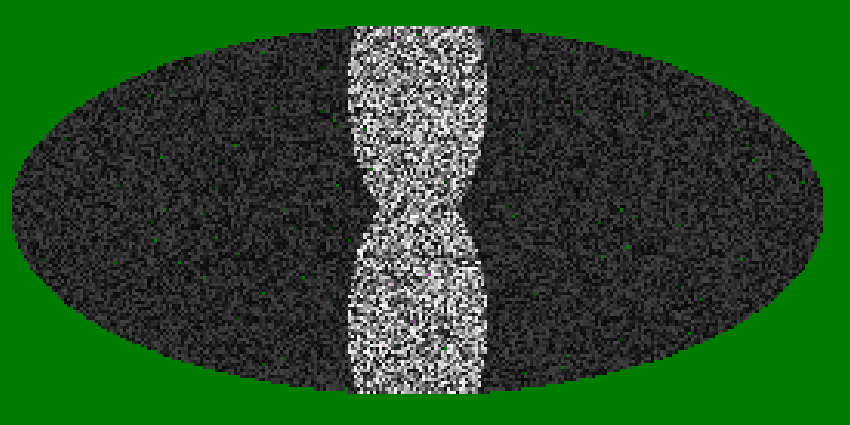
\includegraphics[width=\textwidth]{\Figures/Huc/fantome_cut.png}
        \label{fig:huc:defaut:otsu:fantome:fantome}
    \end{subfigure}
    %
    \begin{subfigure}[b]{0.45\textwidth}
        \caption{Fantome gradienté}
        \centering 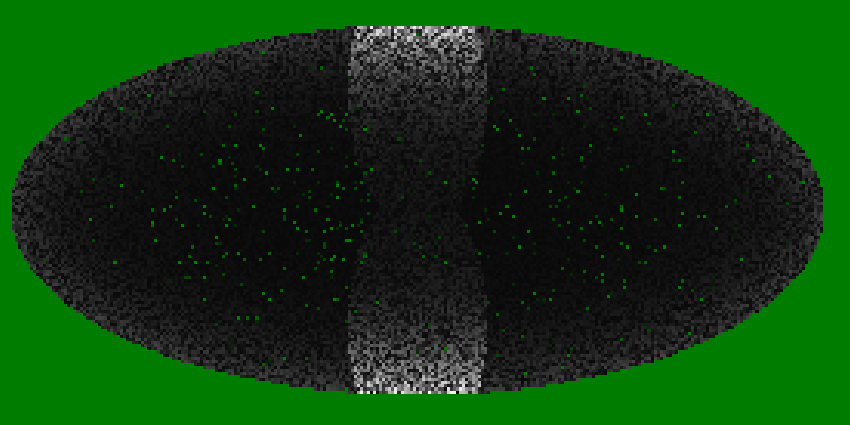
\includegraphics[width=\textwidth]{\Figures/Huc/decay_cut.png}
        \label{fig:huc:defaut:otsu:decay:fantome}
    \end{subfigure}
    %
    \begin{subfigure}[b]{0.45\textwidth} 
        \caption{seuillage du fantôme original}
        \centering 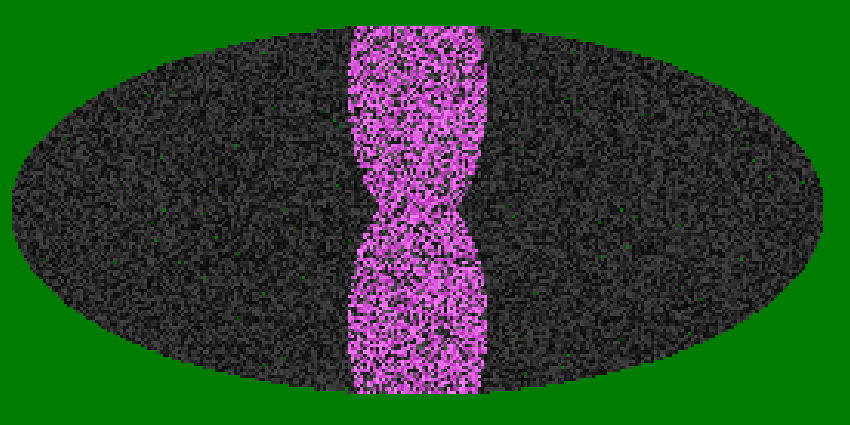
\includegraphics[width=\textwidth]{\Figures/Huc/fantome_otsu_cut.png}
        \label{fig:huc:defaut:otsu:fantome:otsu}
    \end{subfigure}
    %
    \begin{subfigure}[b]{0.45\textwidth} 
        \caption{seuillage du fantôme gradienté}
        \centering 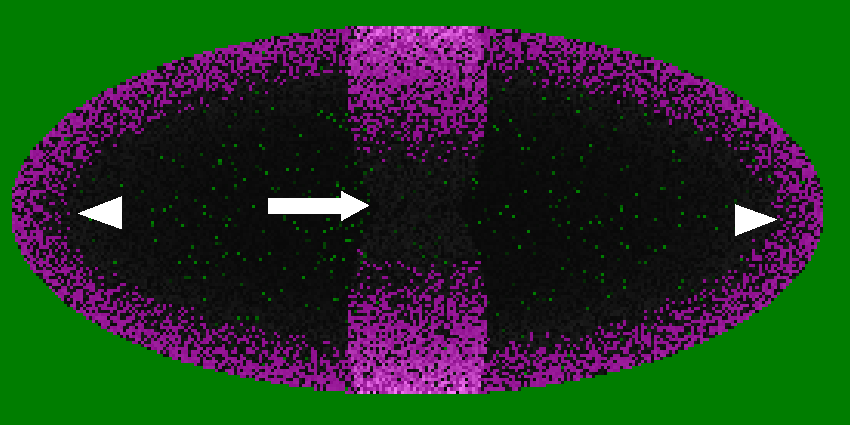
\includegraphics[width=\textwidth]{\Figures/Huc/decay_otsu_cut.png}
        \label{fig:huc:defaut:otsu:decay:otsu}
    \end{subfigure}
    %
    \begin{subfigure}[b]{0.45\textwidth} 
        \caption{Histogramme du fantôme original}
        \centering \includegraphics[width=\textwidth]{\Figures/Huc/fantome_histo.png}
        \label{fig:huc:defaut:otsu:fantome:histo}
    \end{subfigure}
    %
    \begin{subfigure}[b]{0.45\textwidth} 
        \caption{Histogramme du fantôme gradienté}
        \centering \includegraphics[width=\textwidth]{\Figures/Huc/decay_histo.png}
        \label{fig:huc:defaut:otsu:decay:histo}
    \end{subfigure}
    %
    \caption{
        Représentation d'une limite des seuillages d'Otsu
        \newline
        La présence d'un gradient induit une diminution de la valeur seuil(e;f).
        La nouvelle valeur de seuil peut devenir suffisamment basse pour détecter du bruit de fond ((d): têtes de flèche).
        A l'inverse, le signal d'intérêt peut ne plus être détecté si sa valeur passe en dessus de la valeur seuil ((d): flêche).
        \newline
        Les voxels ayant une valeur de gris nulle  sont représentés en vert.
        Les voxels segmentés par seuillage d'Otsu sont représentés en magenta.
        Les barres noires verticales au sein des histogrammes représentent la valeur du critère d'Otsu.
        }
    \label{fig:sblc:defaut:surface}
\end{figure}

%%
%
Un autre défaut est la restriction au plus grand objet de l'image.
%
Imaginons un défaut dans la matière grise qui produirait une séparation entre la partie gauche et la partie droite du cerveau.
%
La réduction au plus grand objet supprimerait alors l'un des deux hémisphères cérébraux.
%
Dans le cas où le volume de la matière grise serait fortement réduit comme chez les mutants homozygotes Fbl (voir \ref{sec:bouffard}),
il est possible que le volume de la matière grise deviennent plus petit que le volume du signal autour du tube digestif, par exemple.
%
De plus, la segmentation de petits élements isolés au sein du cerveaux est ainsi impossible, comme les corps cellulaires se trouvant au sein du toit optique.
%%
%
Afin de supprimer cette étape il serait possible de mettre en place une procédure utilisant la segmentation de la matière blanche.
%
En conservant seulement les objets proches de la segmentation de la matière blanche, il serait alors possible de compenser ce défaut.

\end{document}
